\chapter{Conclusions and Perspectives}\label{chap:conclusion}

As the application of zebrafish in research is becoming more sought after, manual analysis of images has become a bottleneck. This thesis has described a complete framework for the segmentation, quantification, analysis and classification of zebrafish images for ISV and CVP. We also presented methods for ISV and CVP quantification for applications not limited to toxicology analysis. Our results show that ISV and CVP analysis can be used to capture the effect of vascular disruptors. 

Roughly 80,000 industrial chemicals are registered on the US market, and very few of them have been screened for disrupting properties. Thus, development of high throughput screening models that can recognize impacts of toxicity can prove to be very vital. The work presented in this thesis, paves the way for all existing research which has been restricted by analyzing huge amount of data. In conclusion, this work will directly impact the transition from qualitative observation to quantitative measurement of zebrafish by not only providing effective segmentation, but also capturing effective dynamics.


\section{Discussion and Limitations}

Zebrafish being a versatile model, is used in analysis of many biological processes, toxic analysis, and drug screening. Despite the potential of the zebrafish as a model, the actual number of analysis reported is small, involving limited numbers of compounds, with analysis performed manually. Many of the studies reported on zebrafish, focuses on ISV, and yet the research to segment and extract the features from ISV has not taken a lift. The ISVs are particularly interesting because their pattern appears to be established primarily, unlike other vessels such as those of the yolk, brain or retina. Thus, ISVs can give us an initial pathway guidance for capturing dynamics related to growth or environmental cues. 

The key bottleneck restricting these analysis is quantification of the high-throughput experiments, because there are few image analysis methods capable of capturing the complexity ISV. The huge amount of data generated for analysis makes manual analysis a time-inhibiting and error prone process subject to inter-observer variations. Computer-based image processing methods are the only viable way to analyze and quantify the data. Current methods analyze images based on pixel information and thresholding. These methods perform well on clearly resolved objects against a uniform background but often struggle with images that possess information with variable sizes, noise, and heterogeneity across images. This is exemplified in many studies where zebrafish vascular became quantifiable only after manual identification or manual analysis. 

In this work, we focus on developing an integrated image processing methodology to analyze zebrafish embryos post chemical treatment. The pipeline consists of Segmentation of the zebrafish embryo, Region Detection, ISV Extraction, and ISV refinement. We quantify extracted ISV to capture the effect of chemical treatment. A critical issue with the quantitative analysis of zebrafish is that it should be invariant to orientation of zebrafish, and it is highly desirable to have a description that is invariant to noise, intensity
and scales. Our algorithm takes care of this critical issue.

ISV segmentation method perform reasonably well for noisy and blur data (fig. \ref{segISVLim}A and \ref{segISVLim}B). Our method does not perform well for very noisy and blurred ISV (fig. \ref{segISVLim}A and \ref{segISVLim}B near the tail region). Also, ISVs shows immense variation in size. They grow small and thin near the end points, as opposed to center as depicted in figure \ref{segISVLim}D and thin again near head region. Our method is limited by very thin and faded vessels. In figure \ref{segISVLim}D faded vessel does not show in our segmentation. Lastly for figure \ref{segISVLim}C, since ISV curled around zebrafish head, we missed many vessels which does not respond within direction parameters of our method.

\begin{figure}[H] 
 \centering
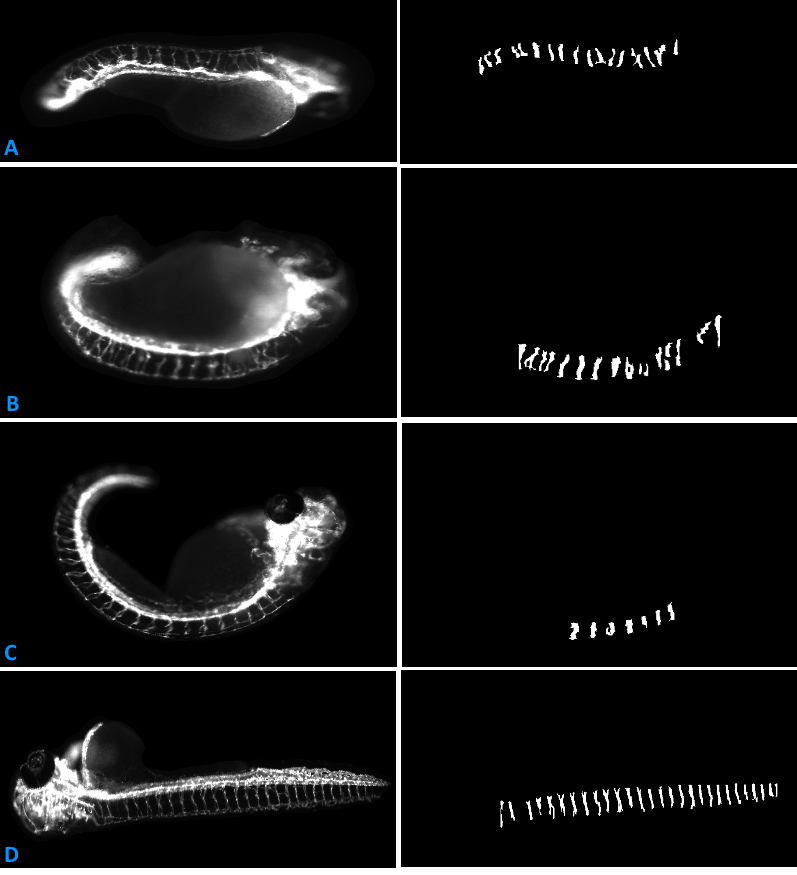
\includegraphics[scale=0.45]{figure/segISVLim.png}
  \caption[Images with the blurred and noisy ISV]{(A), (B) The vessels are more noisy and blurry (C) We lost ISV, due to direction limitation opposed to in tail region. (D) ISVs occur in various sizes, with weak boundary response. Vessels that does not produce a strong response during eigenanlysis also gets excluded during segmentation. Overall, Our algorithm did segmentation of most of ISV. Parameter selection for ISV response and merging causes some loss in data.}
 \label{segISVLim}
\end{figure}



Choice of our parameter effects ISV merging. ISVs remain disjoint is they do not lie within parameter range. In order to negate the effect of direction restriction, we also get response from ISV image in all direction as the probable ISV pixels. Morphological closing operation is applied on direction based ISV and later merged with direction free ISV response. This helps us merge vessels, but if there is no response from direction free ISV, they remain unlinked.

The developed segmentation presents several advantages. Firstly, the parameters are established directly from images so that user interaction is minimal. Secondly, it is not iterative and it can be performed rapidly. Thirdly, this method performs well for images with varied intensity profile and varied texture, orientation and size. Hence, this method possesses the capacity to capture highly dynamic vessels, regardless of phenotype types that exhibit a wide range of morphologies.

We have presented method for segmentation and analysis for CVP. CVP segmentation is based on prior knowledge about change in curvature around tail region. If, our algorithm is not able to find point with the steepest change in curvature, we assume the point where tail starts is the mid point of the curve tracing tail + yolk region. High toxicity impacts the structure of zebrahish, hence perturbing tail region. In those, cases we resort to mid point of curve, which does the good job capturing CVP structure properties. But, it captures more then CVP region (fig. \ref{segISVLim}A, \ref{segISVLim}B, \ref{segISVLim}C). 


\begin{figure}[H] 
 \centering
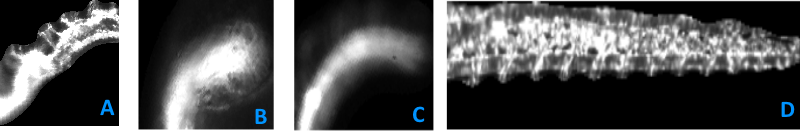
\includegraphics[scale=0.6]{figure/segCVPLim.png}
  \caption[Images with the blurred and noisy CVP]{(A), (B), (C) The tail vessel is structurally damaged due to high dosage. We do get a good estimate of CVP region, but not exact. (D) We are able to segment CVP region well.}
 \label{segCVPLim}
\end{figure}

\section{Future Work}

\textbf{Segmentation}
\newline
In terms of related work, there is a definitely a place for improvement of segmentation of ISV and CVP. Some zebrafish curve around its head under the influence of chemicals. Peng et al. \cite{peng2008} proposed method to straighten curved worm based on formulating the backbone of a worm as a parametric cubic spline defined by a series of control points. This method, can be applied to backbone of zebrafish. This method will improve both the ISV and CVP segmentation.
\textbf{Features}
\newline
Improvement in segmentation, will concurrently improve extracted features. For CVP analysis fusion of morphological properties, with shape properties may improve the classification accuracy. It will be interesting to be able to fuse model for both ISV and CVP to study the toxicology effects and determine safe dosages from chemicals. There is also a scope to be able to extend ISV and CVP analysis algorithm for various other dimensions including 2D + t, 3D, 3D + t. 
\textbf{Applications}
\newline
We have tested our algorithms for application in toxicology. It can be easily extended for drug screening, gene expression modification, or disease modeling. 
% more screen, more applications.

% 
